\chapter{Diseño e implementación} % Main chapter title

Este capítulo presenta la arquitectura del sistema embebido, la estructura de los componentes de software principales, las consideraciones en la selección de componentes electrónicos, y el diseño del PCB y el gabinete del sistema.

\label{Chapter3} % Change X to a consecutive number; for referencing this chapter elsewhere, use \ref{ChapterX}

\definecolor{mygreen}{rgb}{0,0.6,0}
\definecolor{mygray}{rgb}{0.5,0.5,0.5}
\definecolor{mymauve}{rgb}{0.58,0,0.82}

%%%%%%%%%%%%%%%%%%%%%%%%%%%%%%%%%%%%%%%%%%%%%%%%%%%%%%%%%%%%%%%%%%%%%%%%%%%%%
% parámetros para configurar el formato del código en los entornos lstlisting
%%%%%%%%%%%%%%%%%%%%%%%%%%%%%%%%%%%%%%%%%%%%%%%%%%%%%%%%%%%%%%%%%%%%%%%%%%%%%
\lstset{ %
  backgroundcolor=\color{white},   % choose the background color; you must add \usepackage{color} or \usepackage{xcolor}
  basicstyle=\footnotesize,        % the size of the fonts that are used for the code
  breakatwhitespace=false,         % sets if automatic breaks should only happen at whitespace
  breaklines=true,                 % sets automatic line breaking
  captionpos=b,                    % sets the caption-position to bottom
  commentstyle=\color{mygreen},    % comment style
  deletekeywords={...},            % if you want to delete keywords from the given language
  %escapeinside={\%*}{*)},          % if you want to add LaTeX within your code
  %extendedchars=true,              % lets you use non-ASCII characters; for 8-bits encodings only, does not work with UTF-8
  %frame=single,	                % adds a frame around the code
  keepspaces=true,                 % keeps spaces in text, useful for keeping indentation of code (possibly needs columns=flexible)
  keywordstyle=\color{blue},       % keyword style
  language=[ANSI]C,                % the language of the code
  %otherkeywords={*,...},           % if you want to add more keywords to the set
  numbers=left,                    % where to put the line-numbers; possible values are (none, left, right)
  numbersep=5pt,                   % how far the line-numbers are from the code
  numberstyle=\tiny\color{mygray}, % the style that is used for the line-numbers
  rulecolor=\color{black},         % if not set, the frame-color may be changed on line-breaks within not-black text (e.g. comments (green here))
  showspaces=false,                % show spaces everywhere adding particular underscores; it overrides 'showstringspaces'
  showstringspaces=false,          % underline spaces within strings only
  showtabs=false,                  % show tabs within strings adding particular underscores
  stepnumber=1,                    % the step between two line-numbers. If it's 1, each line will be numbered
  stringstyle=\color{mymauve},     % string literal style
  tabsize=2,	                   % sets default tabsize to 2 spaces
  title=\lstname,                  % show the filename of files included with \lstinputlisting; also try caption instead of title
  morecomment=[s]{/*}{*/}
}


%----------------------------------------------------------------------------------------
%	SECTION 1
%----------------------------------------------------------------------------------------
\section{Arquitectura del sistema embebido}

En la Figura \ref{fig:arquitectura_sistema} se muestra un diagrama de bloques con la arquitectura del sistema SCI-CAN y sus interacciones. El recuadro azul, marcado como \textit{controlador}, es lo que corresponde al desarrollo de este trabajo. En los recuadros externos están los dispositivos con los que este sistema debe interactuar: PLCs, servomotores SN-17 y PCs. Con los PLCs, la interacción es a través de señales discretas que necesitan estar correctamente acondicionadas, como se especifica en los requerimientos del trabajo. Con los servomotores, la comunicación es a través de un bus CAN, como se explicó en capítulos previos. La interacción con una PC se consigue meidante el protocolo USB, junto con una adaptación de señal de un conversor.

\begin{figure}[htbp]
	\centering
	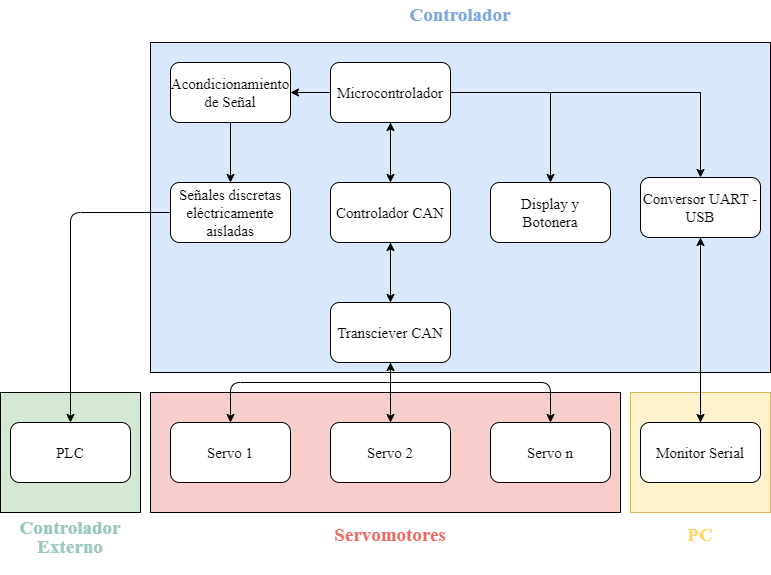
\includegraphics[scale=.5]{./Figures/Arquitectura_SE.png}
	\caption{Arquitectura del sistema}
	\label{fig:arquitectura_sistema}
\end{figure}

Las interacciones internas del sistema incluyen:
\begin{itemize}
	\item Periférico controlador y \textit{transceiver} CAN.
	\item Señales discretas eléctricamente aisladas de la alimentación del sistema.
	\item Display LCD.
	\item Teclado matricial.
	\item Puerto USB.
\end{itemize}

El display y el teclado son las interfaces directas que permiten la interacción de un usuario con el sistema. Como se explicó en el capítulo \ref{Chapter2}, utilizan tanto I2C como entradas y salidas discretas del controlador, respectivamente, para ser manipulados por el microcontrolador. También, en la sección \ref{conversor_usb}, se detalla el funcionamiento de una interfaz UART-USB, utilizada para generar la interacción entre el controlador con una PC externa. Este medio puede ser utilizado como interfaz de usuario con el uso de un software de monitoreo serial en la PC.

\section{Selección de componentes}
\label{seccion_seleccion_componentes}

Previo al desarrollo del hardware y del software, se determinaron los componentes sobre los cuales se construye el trabajo. En su selección, se eligió como proveedor principal a la empresa Digikey\citep{web_digikey} y, para los que se consiguieran dentro de la Argentina, a SyC electrónica\citep{web_syc}. Ambas son empresas con las que Cambre ICyFSA trabaja regularmente. 

En general, se buscó que los componentes tengan las siguientes características:
\begin{itemize}
	\item Disponibilidad en el mercado.
	\item Facilidad para ensamble manual.
	\item Conocimiento previo sobre su uso.
	\item Bajo costo.
\end{itemize}

La disponibilidad de los componentes terminó resultando uno de los problemas principales en el desarrollo del proyecto debido al gran desabastecimiento generado en el transcurso de la pandemia Covid-19. Esto fue una limitante a la hora de realizar la selección.

Algunos de los componentes se eligieron porque ya se había trabajado con ellos para el proyecto SN-17 y se contaba con stock de estos. Entre ellos se puede mencionar el microcontrolador ATSAMC21G18A\citep{web_ATSAMC21G18A}. Este se destaca por ccontar con un periférico controlador CAN incorporado. También por razones de stock y de uso previo se seleccionó el \textit{transceiver} CAN LTC2875IS8\citep{web_transciever_CAN}.

Para el regulador de tensión se seleccionó el LM2575\citep{web_LM2575} con el empaquetado D2PAK. Este es un componente muy popular para este tipo de aplicaciones y presentaba disponibilidad de stock al momento de la elección. Se verificó que cumpliera los requerimientos de alimentación del sistema y se calculó que las temperaturas de operación fueran adecuadas.

Para la interfaz UART-USB, la falta de disponibilidad de opciones resultó especialmente limitante. Se buscó un modelo que el fabricante indicara que era reconocido por Windows y sus drivers instalados de forma automática, para facilitar el uso del dispositivo. Se seleccionó el integrado CY7C64225\citep{web_interfaz_USB_UART}.

Con respecto a los optoacopladores, se estudiaron aquellos que cumplieran con el requerimiento de aislación eléctrica de 1 kV, que fueran de 4 canales y que su \textit{footprint} fuera el menor posible. Se eligió el LTV-846S\citep{web_optoacopladores_LTV}.

Una vez seleccionados todos los componentes principales del sistema, se estudiaron los datasheets y se seleccionaron los componentes periféricos indicados en estos. Con esta información se completó el listado de componentes del sistema y se prosiguió con su adquisición.

Para el display LCD se eligió uno similar al explicado en la sección \ref{seccion_display_led} del cual se contaba con amplia disponibilidad en el mercado local. Este trae incorporado la interfaz I2C para su manipulación.

Para el teclado matricial se buscó un modelo que tuviera cierta robustez mecánica en su composición, y que tuviera un tamaño similar al display. Se eligió el que se muestra en la Figura \ref{fig:keypad}, que es de 4 filas y 4 columnas, del fabricante Adafruit\citep{web_adafruit}.

\begin{figure}[htbp]
	\centering
	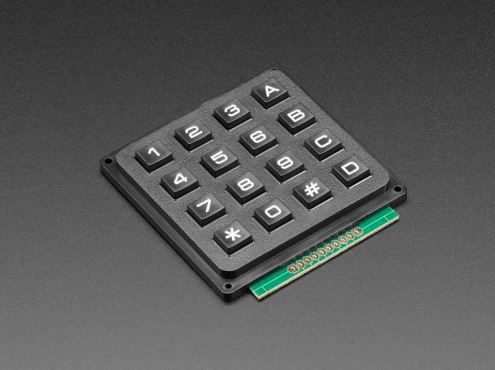
\includegraphics[scale=.8]{./Figures/keypad.JPG}
	\caption{Teclado matricial Adafruit 4x4\citep{web_keypad}}
	\label{fig:keypad}
\end{figure}



\section{Comunicación CAN}
\label{comunicacion_can}

La implementación de una red CAN requiere consideraciones de diseño relacionadas con el \textit{bitrate} y los tiempos de bit con los cuales trabaja el protocolo para la lectura y envío de información. Como se explicó en la sección \ref{caracteristicas_can}, estas variables están relacionadas a la longitud del bus y al ruido eléctrico al que está expuesto. En la Figura \ref{fig:bit_times} se presentan los tiempos de bit recomendados para implementaciones de CANopen\citep{Understanding_CAN}. De este listado se seleccionó la fila para un bus de 250 m, que recomienda un \textit{bitrate} de 250 kb/s y los tiempos de bit correspondientes. Esto se configura en el periférico de CAN del microcontrolador.

\begin{figure}[htbp]
	\centering
	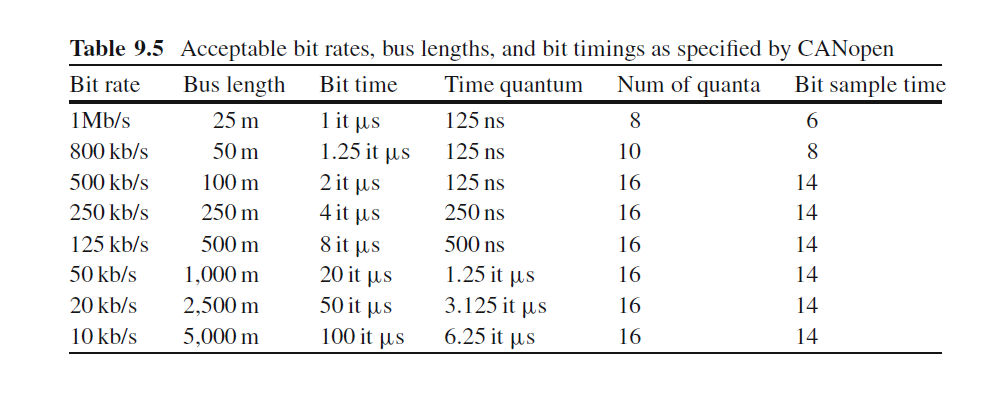
\includegraphics[scale=.5]{./Figures/bit_times_recomendados.PNG}
	\caption{Tiempos de bit recomendados para CANopen}
	\label{fig:bit_times}
\end{figure}

La estructura en la que se codificó la información dentro de los mensajes CAN se muestra en la Figura \ref{fig:estructura_mensajes}. Se utilizó tanto el campo de identificador estándar de 11 bits como los bytes de data para indicar el tipo de mensaje y la manera en que debe ser procesado.

En el campo de identificador se empleó el primer bit para indicar si el mensaje es un error. Dentro de la red, todos los mensajes que tengan este bit encendido no son filtrados y son los que tienen la mayor prioridad. Los siguientes 9 bits indican el identificador del dispositivo transmisor o receptor del mensaje, según corresponda. Cada dispositivo en la red tiene un número identificatorio único, el cual es fijo en el firmware. También, se especifican identificadores comunes para mensajes del tipo \textit{broadcast}, dirigidos a todos los dispositivos de la red. El último bit se usa para indicar la dirección del mensaje, es decir, si es un mensaje envíado por el SCI-CAN, que actúa como dispositivo central de la red, o por un sistema SN-17.

\begin{figure}[htbp]
	\centering
	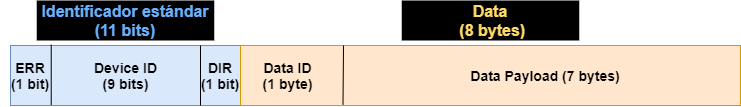
\includegraphics[scale=.5]{./Figures/estructura_mensaje.png}
	\caption{Estructura de mensajes CAN}
	\label{fig:estructura_mensajes}
\end{figure}

Eel campo de data tiene una longitud total de 8 bytes. El primer byte se utiliza para identificar el tipo de información del mensaje, mediante un \textit{data ID}. En la Tabla \ref{tab:tipos_mensajes_CAN} se muestran todos los \textit{data ID} implementados en el sistema y el carácter de esa información. Para cada uno de estos tipos de mensaje la información se codifica de una forma diferente. Distintas funciones debieron ser desarrolladas en el software para su implementación, como se explica en las secciones siguientes.

\begin{table}[h]
	\centering
	\caption[Operaciones SN-17]{Funciones de SN-17}
	\begin{tabular}{c c c}    
		\toprule
		\textbf{\textit{Data ID}} 	& \textbf{Tipo}  & \textbf{Descripción}\\
		\midrule
		Tipo de instrucción & Instrucción 	& Define la instrucción\\		
		Límite de torque 	& Instrucción	& Torque máximo de instrucción \\
		Modo de control		& Instrucción 	& Posición, velocidad, torque \\
		\textit{Set point}	& Instrucción 	& Valor de lazo de control \\
		\textit{Threshold}	& Instrucción 	& Valor de error admisible \\
		\textit{Hold time}	& Instrucción 	& Tiempo de cumplimiento \\
		\textit{Timeout}	& Instrucción 	& Tiempo de no cumplimiento \\
		Guardar posición	& Configuración & Guarda posición actual \\
		Calibrar posición	& Configuración & Guarda posición manual \\
		Constantes PID		& Configuración & Constantes lazo de control \\	
		Entradas y salidas	& Configuración & Funcionamiento de las IO \\
		\textit{Homing}		& Configuración & Establece rutina de cerado \\	
		Calibración			& Comando		& Inicia la rutina de calibración \\
		Activar motor		& Comando		& Enciende/apaga el motor \\		
		\textit{Go Home}	& Comando		& Inicia la rutina de cerado \\		
		Mover motor			& Comando		& Rota un ángulo específico\\
		Rotar motor			& Comando		& Gira a velocidad específica \\
		Torquear motor		& Comando		& Gira a torque específico \\
		Límite torque manual& Comando		& Limita el torque de comandos \\
		Activar salidas		& Comando		& Enciende/apaga salidas \\	
		Consultar motor		& Comando		& Consulta información del motor \\
		Programa manual		& Comando		& Corre un programa en modo maual \\
		Instrucción actual	& Supervisión	& Instrucción ejecutada del motor \\
		Encoder				& Supervisión	& Posición de encoder del motor \\
		Error				& Supervisión	& Tipo de error del motor \\
		Cambio de modo		& General		& Programación o operación \\
		\textit{Device ID}	& General		& Consulta de IDs de red \\
		\bottomrule
		\hline
	\end{tabular}
	\label{tab:tipos_mensajes_CAN}
\end{table}

Los mensajes del tipo instrucción se refieren a las instrucciones de los programas que ejecutan los sistemas SN-17 en operación. Codifican un número según el tipo de dato que se utilice y el número de programa e instrucción al que corresponden. Para los mensajes de configuración, se agrega información complementaria en cada uno para indicar los parámetros configurables. Por ejemplo, en el caso de una constante PID, se indica en forma codificada cual es la constante en cuestión y el valor de esta. Tanto las señales de instrucción como de configuración pueden tener ambas direcciones de transmisión según si es una programación o una consulta.

Los mensajes de comando se caracterizan en que son envíados exclusivamente por el SCI-CAN para exigir la ejecución de alguna operación de los motores. Como en el caso de las configuraciones, algunos comandos requieren de información complementaria que se codifica en los bytes de \textit{payload}, según sea necesario.

Los mensajes de supervisión son envíados exclusivamente por los motores cuando se encuentran en modo de operación y se usan para indicar el estado actual de funcionamiento de estos.

Finalmente, los mensajes del tipo general son envíados por la central como \textit{broadcast} para todos los dispositivos de la red, los cuales responden usando el mismo identificador. Estos mensajes se usan para controlar el funcionamiento general de la red.

VER SI EN ESTA SECCION CONVIENE AGREGAR MAS GRAFICOS O TABLAS PARA DESCRIBIR EN MAYOR DETALLE LA CONFORMACION DE CADA UNO DE LOS MENSAJES. QUIZAS UNA TABLA INDICANDO CADA UNO DE LOS 8 BYTES SEGUN ID

\section{Desarrollo de software}
\label{desarrollo_software}

\subsection{Arquitectura de Software}

El desarrollo del software se realizó sobre una placa de evaluación del microcontrolador seleccionado\citep{web_dev_board}. Esto permitió hacer pruebas del sistema previo al diseño del circuito, lo que facilitó el proceso de implementación.

El software del sistema se diagramó siguiendo una estructura de capas. En la Figura \ref{fig:arq_software} se muestra un esquema de la arquitectura de software implementada. Como se puede observar, las capas intermedias interactúan con la capa superior de aplicación mediante el uso de servicios públicos que cada uno de los manejadores ofrece. Las capas inferiores (Key, LCD I2C handler, buffer circular) no son visibles por la capa de aplicación, pero ofrecen funcionalidades para las capas intermedias. 

\begin{figure}[htbp]
	\centering
	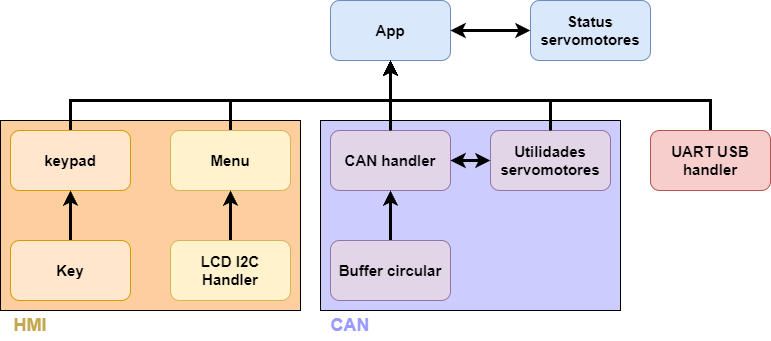
\includegraphics[scale=.5]{./Figures/arquitectura_software.png}
	\caption{Arquitectura de software}
	\label{fig:arq_software}
\end{figure}

En la capa superior se tiene a la aplicación, que interactúa, en un mismo nivel, con una sección del código que almacena el status de los distintos servomotores. En esta capa de software se coordina el funcionamiento e interacción de las capas intermedias.

El recuadro marcado como HMI (\textit{Human Machine Interface}) se relaciona con la sección del programa encargada de proveer la interfaz de usuario. Maneja las acciones del teclado matricial y la información que se visualiza en el display.

La sección CAN se relaciona con las configuraciones del periférico controlador del protocolo, las funciones para codificar los mensajes, el envío y recepción de mensajes y los servicios ofrecidos por los servomotores.

El manejador de UART-USB es el encargado de las interacciones con una PC. Realiza la codificación de información de los mensajes y procesa los datos recibidos por el puerto USB. 

En las subsecciones siguientes se explica el desarrollo de estos componentes principales del software implementado.

\subsection{Driver CAN}

Para la implementación del módulo CAN handler de la Figura \ref{fig:arq_software} se utilizó el periférico de este protocolo de comunicación que contiene el microcontrolador seleccionado. Se configuró mediante la herramienta de desarrollo provista por el fabricante\citep{web_microchip_studio}, a través de la cual se seleccionaron:
\begin{itemize}
	\item Los tiempos de bit y la tasa de transmisión de 250 kb/s, según la Figura \ref{bit_times}.
	\item El uso del identificador estándar.
	\item El funcionamiento de los filtros.
	\item La operación en caso de colisiones.
\end{itemize}

El driver implementado opera por interrupción, con funciones de \textit{callback} que son llamadas cuando se recibe o termina la transmisión de un mensaje. Para esto, se adaptó el código de ejemplo provisto por el fabricante.

Para la recepción de mensajes, se empleó un módulo de software de \textit{buffer} circular, adaptado del trabajo final de especialización de Gabriel Gavinowich\citep{tpf_gabriel}. Este permite el almacenaje de más de un mensaje y evita que esta información se pierda en caso de que el procesador se encuentre ocupado atendiendo otra tarea y llegue un nuevo mensaje en el bus. Los mensajes que se encuentran almacenados en el \textit{buffer} son luego procesados fuera del estado de interrupción, dentro del ciclo del bucle principal.

Para la interpretación de los mensajes, se construyó el módulo de software marcado como \textit{Utilidades servomotores} en la Figura \ref{fig:arq_software}. Dentro de este, se implementaron distintas funciones locales que decodifican el identificador y la data según el tipo de mensaje. 

Con identificador CAN se determina si el mensaje recibido indica un error (primer bit) y si está dirigido a un SN-17 o al SCI-CAN (último bit de dirección). Con respecto a la información del tipo, como se explicó en la sección \ref{comunicacion_can}, esta se encuentra codificada en el primer byte de data del mensaje CAN. Esta es identificada y, utilizando una estructura \textit{switch-case}, se selecciona la función decodificadora correspondiente.

VER SI SE PUEDE AGREGAR UNA IMAGEN PARA CLARIFICAR EL CONCEPTO DEL CODIGO

ESCRIBIR SERVICIOS A CAPAS SUPERIORES 

\subsection{Interfaz HMI}

La interfaz HMI involucra la interacción del software del sistema con el teclado y con el display LCD. Su implementación implicó el desarrollo de los drivers de I2C, para comunicarse con la pantalla, y del teclado, un \textit{middleware} que controle un sistema de menúes, la interacción de ambos drivers y que ofrezca funcionalidades a la capa superior de aplicación.

Con respecto al driver I2C para el display, para la configuración del protocolo se empleó la herramienta de desarrollo ofrecida por el fabricante del microcontrolador. Sobre eso, se construyeron una serie de servicios para mostrar información en el display siguiendo ejemplos de códigos libres de implementaciones sobre Arduino\citep{web_arduino} de este tipo de dispositivos\footnote{https://github.com/fdebrabander/Arduino-LiquidCrystal-I2C-library}.

Para el driver del teclado\footnote{https://github.com/Chris--A/Keypad}, se siguió una metodología similar, usando la herramienta de desarrollo para hacer la configuración de los pines de entradas y salidas del controlador y, sobre eso, se implementó una estructura de código adaptada de implementaciones libres de Arduino que ofrecen servicios para reconocer que teclas se oprimieron a capas superiores.

Sobre estos manejadores, se desarrolló un software que utiliza a ambos para generar el sistema de menúes y su interacción con un usuario. Mediante el uso del teclado se puede navegar a través de una lista de opciones que se muestran en el display y se permite visualizar y configurar los parámetros de los motores conectados. En la Figura \ref{fig:menu} se muestra un ejemplo de cómo se presentan las opciones en el display. La flecha presente a la izquierda de la imagen es la que le permite al usuario ubicarse a medida que se navega por los menúes con la utilización del teclado.

\begin{figure}[htbp]
	\centering
	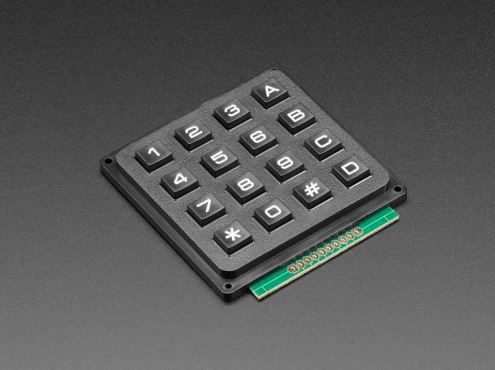
\includegraphics[scale=.6]{./Figures/keypad.JPG}
	\caption{Ejemplo de opciones de menú - ARMAR IMAGEN}
	\label{fig:menu}
\end{figure}

Se planteó que el menú cuente con 2 pantallas diferentes según el estado en el que esté: monitoreo o programación. En el estado de monitoreo, se muestra una primera pantalla donde puede observarse el programa e instrucción que cada motor conectado está ejecutando en ese momento y puede navegarse para consultar la configuración, pero esta no puede ser modificada.

En el estado de programación, la configuración de los distintos motores es accesible para ser modificada y, además, se muestran los distintos comandos manuales que pueden ejecutarse para cada motor. Al pasar del estado de monitoreo al de programación, la central envía un mensaje de \textit{broadcast} usando un ID prioritario a la red al que cada motor responde con su ID particular.

El software de menúes le indica a la capa superior de aplicación la acción solicitada por el usuario, y es esta capa la que interactúa con los otros drivers, como se explicó en la sección \ref{desarrollo_software}.

\subsection{Interfaz UART-USB}

La interfaz UART-USB involucró el desarrollo de un manejador de UART desde el microcontrolador. Para esto, se utilizó la herramienta de desarrollo provista por el fabricante, donde se realizó la configuración del periférico de comunicación. El software opera por interrupciones de hardware, que llaman a funciones de \textit{callback} al completar una transmisión o recepción de mensaje.

Los mensajes UART son adaptados a señales USB mediante el circuito integrado CY7C64225\citep{web_interfaz_USB_UART}. Esto permite la conexión del dispositivo con un monitor serial en una PC.

Sobre este manejador UART se construyó una herramienta de reporte que se ejecuta en la capa de aplicación que envía las acciones seleccionadas por el menú a través de USB. Esto permite confirmar que la información seleccionada es la correcta y facilita la detección de errores.

También, se puede utilizar una PC para enviar data al dispositivo, para que este lo transmita a un motor conectado. Esto se implementó utilizando la misma estructura de mensajes de CAN, los cuales se envían desde una conexión serial y el dispositivo los convierte a señales CAN directamente.  

\section{Modificaciones firmware SN-17}

Para que el sistema SCI-CAN pueda comunicarse con las plaquetas SN-17, se tuvieron que realizar modificaciones al firmware de estas. Estos cambios tuvieron 3 objetivos principales:
\begin{itemize}
	\item Incorporar los drivers de CAN y la estructura de mensajes planteada.
	\item Generar que las configuraciones y programas sean variables modificables.
	\item Lograr el almacenado de las configuraciones en memoria no volátil.
\end{itemize}

Con respecto a la implementación de CAN, los módulos de software desarrollados para el SCI-CAN se utilizaron en los sistemas SN-17, sin modificaciones. Esto fue posible debido a que ambos sistemas utilizan el mismo microcontrolador. Siguiendo la estructura de CAN de la Figura \ref{fig:arq_software}, los módulos de CAN handler y buffer circular se mantuvieron idénticos para ambos sistemas.

Para la implementación del módulo de utilidades de servomotores se buscó también que ambos sistemas compartieran el mismo software. Para ello, se planteó el uso de sentencias condicionales que determinaran si un mensaje está dirigido a un sistema SCI-CAN o a un SN-17. A partir de esto, se determina la acción a realizar en la capa de aplicación según la información del mensaje. En el caso de un sistema SN-17, la capa de aplicación recibe de la capa CAN la solicitud de realizar determinada acción, la cual procesa según corresponda.

Para lograr que las configuraciones y los programas del sistema SN-17 sean modificables sin necesidad de cambiar el firmware, se utilizó una estructura para almacenar esta información. Esta estructura es accedida directamente por la capa de aplicación, quien se encarga de administrarla. 

Esta misma estructura se aplicó en el dispositivo SCI-CAN, donde se utilizan varias instancias de esta para almacenar la información reportada por los sistemas SN-17 conectados a la red. En el esquema de la Figura \ref{fig:arq_software}, el módulo Status servomotores es el que implementa la estructura descripta. La misma arquitectura es empleada en los sistemas SN-17, con la diferencia de que cuentan con una única instancia de la estructura de información.

VER DE AGREGAR ACA UNA IMAGEN EXPLICANDO LA INFORMACION DE LA ESTRUCTURA.

Para el almacenaje, se utilizó la misma estructura de información del sistema. El microcontrolador empleado permite la escritura de algunas secciones de memoria no volátil interna mientras el dispositivo se encuentra en operación. Sin embargo, estas secciones se comparten con el firmware del dispositivo, por lo que es necesario determinar correctamente las secciones disponibles. Para esto, se modificó el archivo \textit{linker script}, donde se indica al compilador el tamaño se la memoria ROM. Esta modificación no permite que el firmware se almacene en cierta sección de la memoria. En esta sección es donde se almacena la información del sistema en tiempo de ejecución.

\section{Desarrollo de Hardware}
\label{desarrollo_hw}

Para el desarrollo del hardware se utilizó el software de diseño Altium Designer\citep{web_altium} y se eligió como fabricante a PCBWING\citep{web_pcbwing} que es una empresa con la que regularmente trabaja Cambre ICyFSA. Se tomó, como punto de partida, las capacidades técnicas de este fabricante.

Se decidió hacer una placa de 4 capas, con dimensiones menores a 100 x 100 mm. Esto se debe a que el fabricante ofrece precios más económicos para estas especificaciones y se consideró que no imponen restricciones importantes el diseño requerido.

Previo al comienzo del desarrollo del circuito esquemático, se recopiló la información de todos los componentes seleccionados y se cargaron sus \textit{pinouts, footprints} y modelos 3D. 

Para los conexionados se seleccionaron los conectores tipo COMBICON con tornillo\citep{web_combicon} para las conexiones externas, y los conectores tipo XH\citep{web_xh_connector} para las conexiones internas del sistema.

El primer paso del diseño fue determinar los subcircuitos del sistema. Estos son:
\begin{itemize}
	\item Microcontrolador
	\item Regulador de tensión	
	\item Interfaz CAN
	\item Entradas discretas
	\item Salidas discretas
	\item Interfaz UART-USB
\end{itemize}

Para cada uno de estos subcircuitos se armó un dibujo esquemático. En la Figura \ref{fig:esquematico_can} puede verse el correspondiente a la interfaz CAN donde se muestra el \textit{transceiver} elegido y sus conexiones. Para cada uno de los componentes principales del sistema, se siguieron las recomendaciones indicadas en la hoja de datos correspondiente. 

\begin{figure}[htbp]
	\centering
	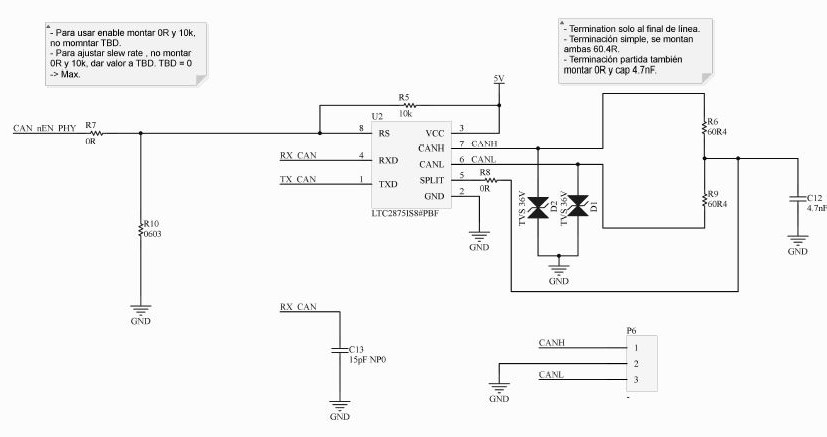
\includegraphics[scale=.6]{./Figures/sch_can.JPG}
	\caption{Esquemático de Interfaz CAN}
	\label{fig:esquematico_can}
\end{figure}

Finalizados los subcircuitos esquemáticos, se continuó al desarrollo del PCB. Primero, se determinaron las dimensiones de la plaqueta, manteniendo las restricciones impuestas y asegurando una cómoda posición de todos los componentes para permitir un ensamble manual. Se eligió a una dimensión final de plaqueta de 100 x 80 mm. 

Para el diseño del \textit{PCB} se buscó que:
\begin{itemize}
	\item Los subcircuitos quedaran separados.
	\item Los conectores quedaran todos en los extermos de la plaqueta.
	\item Se respetara la aislación eléctrica de las entradas y salidas con el circuito de control.
	\item Se minimizara la longitud de las líneas de CAN y se maximizara su simetría.
\end{itemize}

La Figura \ref{fig:render_pcb} muestra el render 3D del \textit{PCB} obtenido. En la parte superior se encuentran los circuitos de entradas y salidas industriales, eléctricamente aislados por los optoacopladores y separados del resto del circuito. En la esquina inferior izquierda, se encuentra el regulador de tensión de 5 V. En el centro, el microcontrolador y, a la derecha, el circuito de CAN y de USB.

\begin{figure}[htbp]
	\centering
	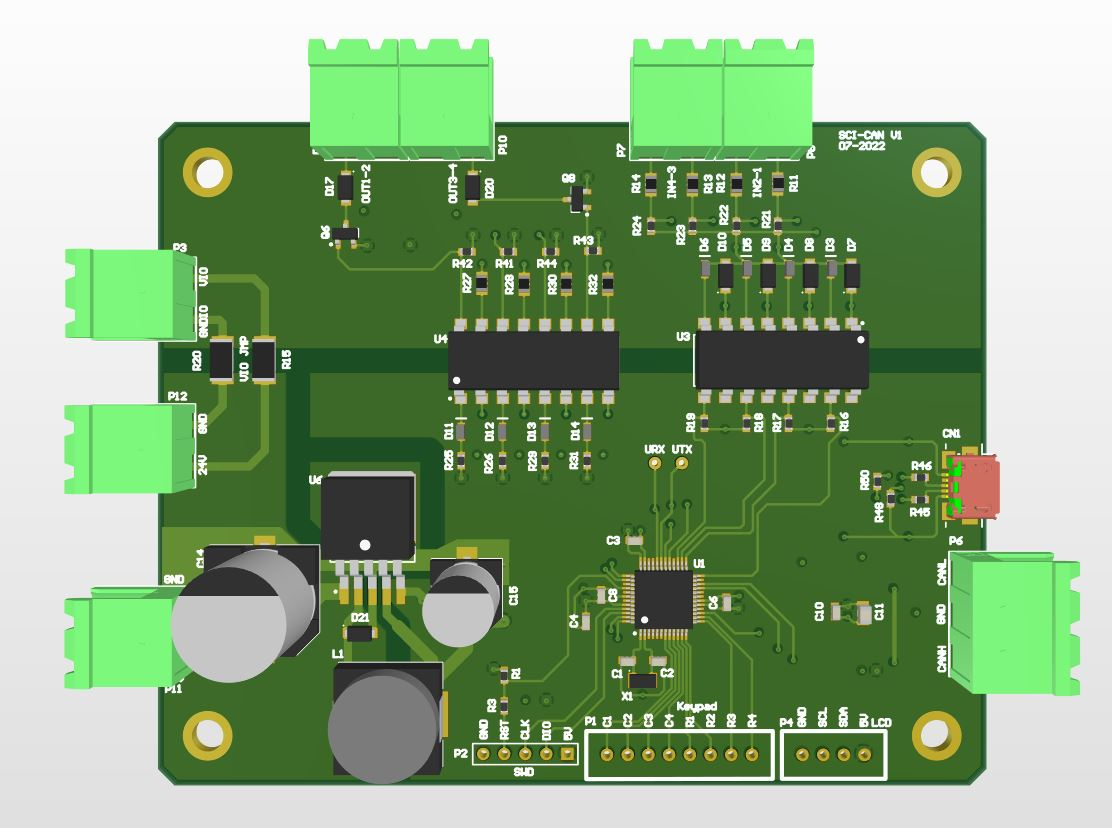
\includegraphics[scale=.4]{./Figures/pcb_sch.JPG}
	\caption{Render del \textit{PCB}}
	\label{fig:render_pcb}
\end{figure}

\section{Desarrollo de gabinete}

Para el desarrollo del gabinete se usó el software de diseño mecánico Autodesk Inventor\citep{web_inventor}. Se determinó armar un ensamble que incluya todos los componentes y se lo pensó para poder luego ser impreso en 3D.

Para los componentes adquiridos, como la pantalla LCD y la matriz de botones, se tomaron los modelos 3D de uso libre de la plataforma GrabCAD\citep{web_grabcad}. Estos se verificaron para asegurarse que sus medidas correspondieran con el dispositivo físico adquirido. El modelo de la plaqueta electrónica SCI-CAN desarrollada se exportó desde el software Altium.

Una vez obtenidos los modelos de estos componentes, se realizó el desarrollo de las distintas piezas que conforman el gabinete. Como consideraciones del diseño se planteó:

\begin{itemize}
	\item Facilitar el acceso a los conectores de la plaqueta SCI-CAN.
	\item Proteger los circuitos internos de la plaqueta SCI-CAN.
	\item Presentar el teclado y el display de forma contigua.
	\item Esconder dentro del gabinete las conexiones entre el display y el teclado con la plaqueta SCI-CAN.
	\item Minimizar la cantidad de partes y de ajustes necesarios.
	\item Limitar los ajustes a roscas métricas.
\end{itemize}

Como restricción adicional de diseño, se tuvieron que mantener las dimensiones máximas de las piezas a medidas menores que la capacidad de fabricación de la impresora 3D \textit{Creality Ender-3}\citep{web_ender3}. Esto corresponde a 220 x 220 x 250 mm.

En la Figura \ref{fig:ensamble} se presenta una imagen del ensamble desarrollado tomada de Inventor. Es importante notar que las piezas superiores, donde están la pantalla y el teclado, se muestran transparentes para facilitar la visualización. Como se puede ver, el ensamble consta de 3 componentes: una tapa delantera donde apoyan el display y el teclado, una caja intermedia que encierra a estos, y una caja trasera donde se coloca la plaqueta de control.

\begin{figure}[htbp]
	\centering
	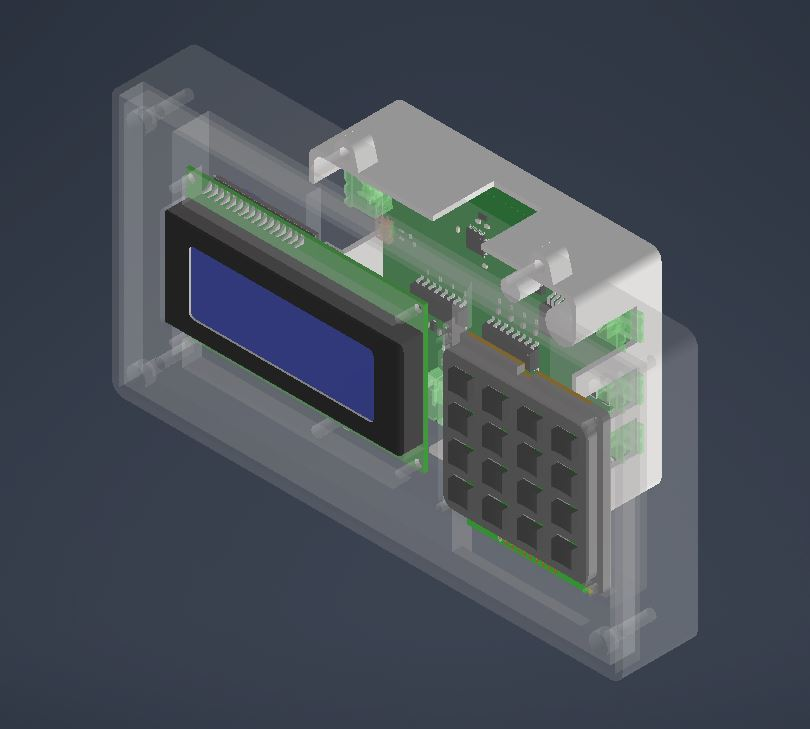
\includegraphics[scale=.6]{./Figures/asm_3d.JPG}
	\caption{Ensamble 3D de gabinete}
	\label{fig:ensamble}
\end{figure}

Para la fabricación del conjunto, se utilizó el programa UltiMaker Cura\citep{web_cura3d}, donde se generaron los archivos de fabricación para impresión 3D. Se decidió utilizar como material PLA, que es uno de los plásticos más económicos y simples de manipular, y que cuenta con las características mecánicas apropiadas para la aplicación.